\subsection{Evaluation Set-up}

% \begin{figure}
%     \centering
%     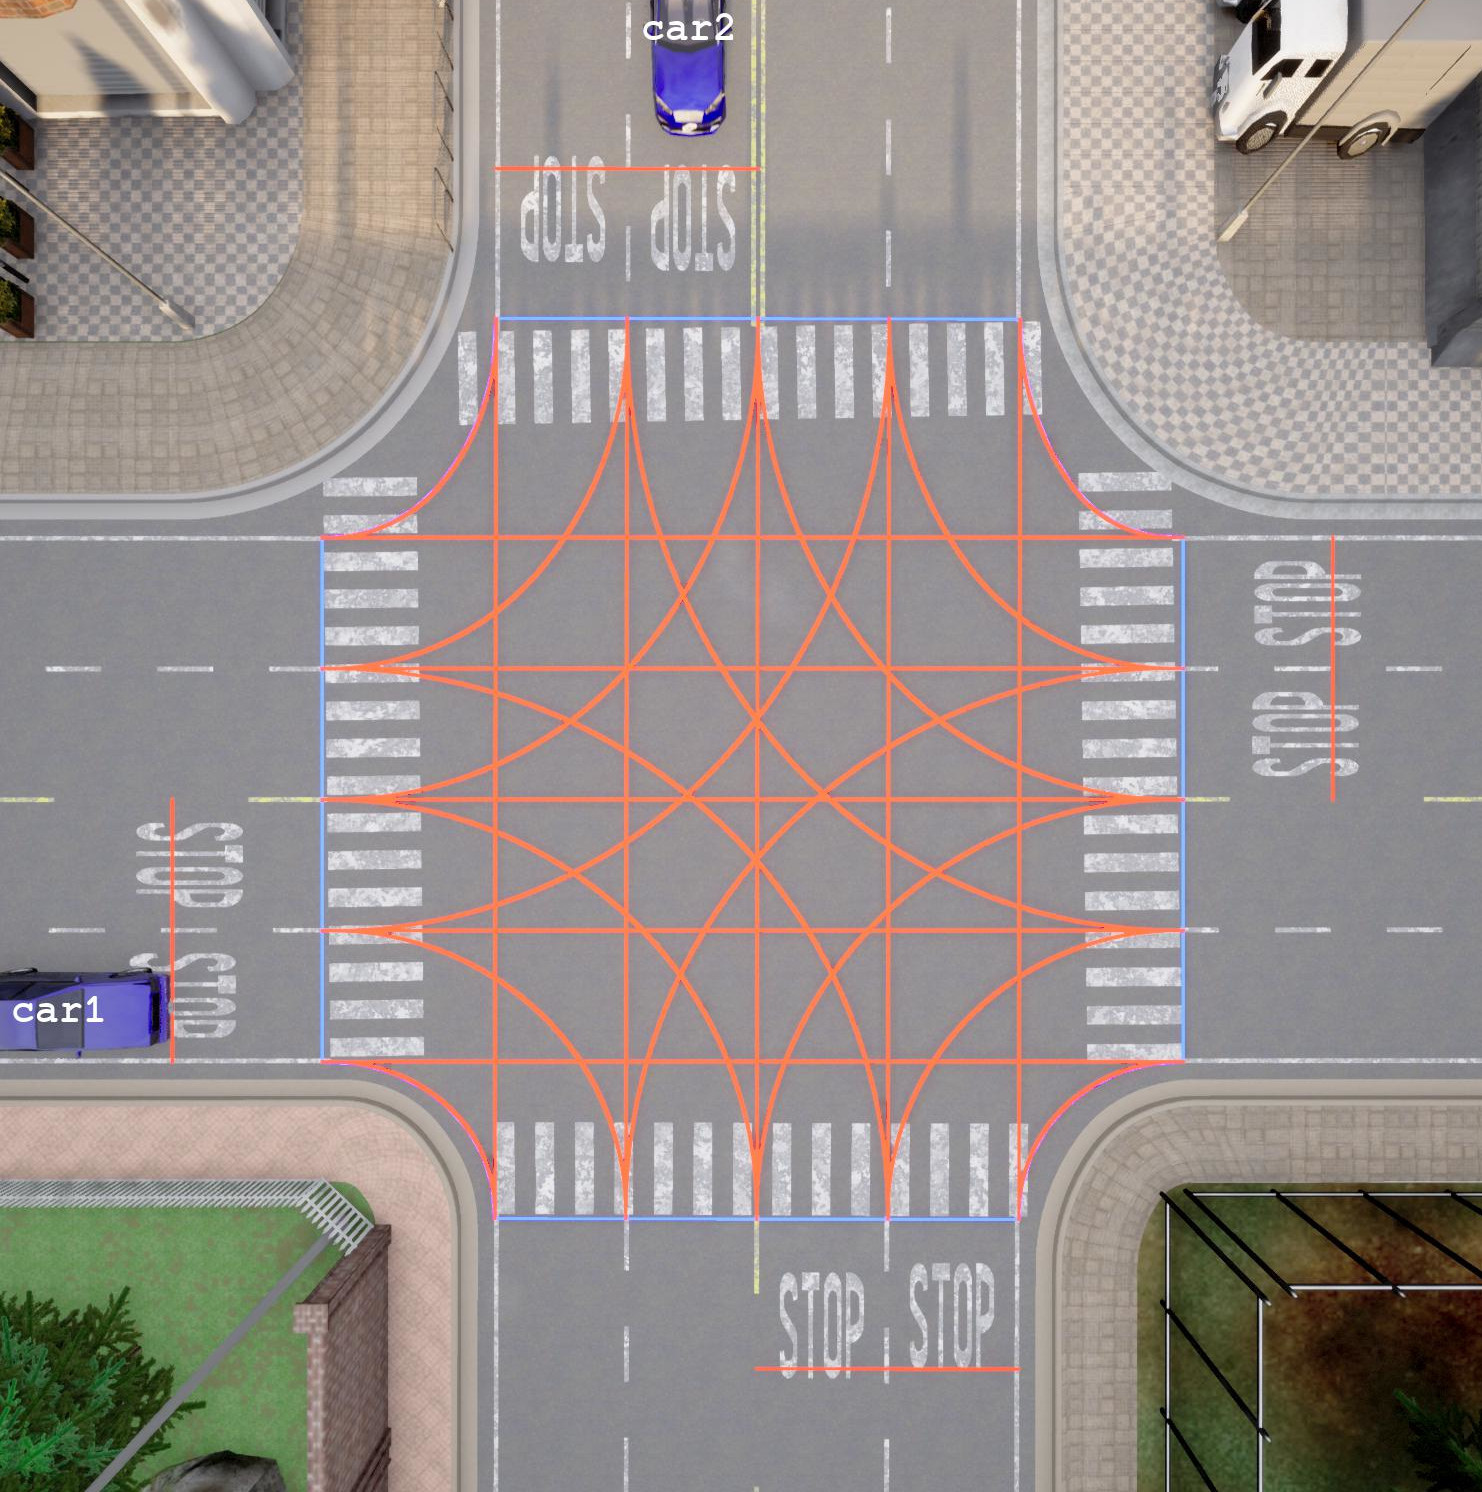
\includegraphics[width=50mm]{figures/4way-stopOnAll.jpg}
%     \caption{Multi-lane four-way stop}
%     \label{fig:4way-stopOnAll}
% \end{figure}

For evaluating the effectiveness of fuzzing in generating a diverse set of inputs, we consider a multi-lane four-way intersection, with two incoming lanes and two outgoing lanes from each side, such as the one provided in Figure~\ref{fig:4way-stopOnAll}.
% 
Considering that a scenario can have several cars waiting to enter and exit the intersection at different points of time, one can think of various scenarios.
% 
Each scenario can have at most one ego vehicle (that implements autonomous driving software) and several non-ego vehicles whose trajectories are generated algorithmically.
% 
The number of non-ego vehicles, the path prescribed to each non-ego, and the velocity profile of each non-ego vehicle is generated by the fuzzer.
% 
As mentioned earlier, since bit-level fuzzing of a scenario description most likely does not yield in a new valid scenario, we use structure-aware fuzzing where we provide custom mutators for manipulating vehicle routes, velocity profiles, etc.
% 
Once the fuzzing algorithm generates a scenario, the scenario is evaluated in a photo-realistic simulator such as CARLA.
% 
We collect the valuations of all the predicates during the scenario to calculate its predicate coverage.
% 
\emph{The predicate coverage metric is the number of unique predicate valuations.}
% 

% The predicates encountered by the ego-vehicle while navigated through the scenario are recorded and used for evaluating the predicate coverage.

%------------------------------------------------------
\subsubsection{Scenario Encoding}
A \emph{test-case scenario} consists of one or more \emph{non-ego} vehicles, and an \emph{ego} vehicle.
%
The trajectories of non-ego vehicles are predetermined at test-case generation time.
%
A test-case specifies the initial position of the ego vehicle while the rest of the trajectory is generated at test-case execution time when an ego \emph{agent} drives the ego vehicle.
%
The ego vehicle is expected to follow a \emph{route} as specified by the test-case, also called ego's \emph{mission}.
%
Each vehicle is associated with a vehicle model, which specifies its shape and dynamics.
%
Each non-ego trajectory is specified using two polynomial splines: \emph{footprint} and \emph{timing}.
%
A \emph{footprint} spline specifies the positions of a vehicle parameterized by travelled distance.
%
The \emph{timing} spline specifies the travelled distance of a vehicle parameterized by simulation time.
%
The \emph{local control property} of splines allows mutators to change a trajectory locally (in location or time) by mutating the splines' control points.
%
This allows local search in the space of trajectories, which is the motivation behind our scenario encoding design.
%
A test-case also specifies the turn-signal events of each non-ego, as a list of pairs of (time, turn signal).


%------------------------------------------------------
\subsubsection{Seeds}

The initial fuzzing seeds are randomly sampled using a probabilistic programming language called SCENIC \cite{Fremont.2020}.
%
A SCENIC scenario specifies a distribution over scenarios, and SCENIC's generator samples from this distribution.
%
The number of vehicles and their initial positions are first sampled to create an \emph{initial scene}.
%
Then each vehicle is driven by an agent to generate vehicle trajectories.
%
One of the vehicles is designated as the ego vehicle.
%
The trajectories of non-ego vehicles are converted to our spline encoding using SciPy's spline approximation.
%
The trajectory of the ego vehicle is used to assign ego's route (mission), i.e. the expected lanes to follow.
%
We keep sampling from the SCENIC scenario for 20 minutes, resulting in 22 seeds.

%-----------------------------------------
\subsubsection{Mutators}
Since a traffic scenario is highly structured and constrained, we use structure-aware mutators.
%
That is, instead of mutating the bit-level representation of a fuzz-input,
the python-object representation of a test-case scenario is mutated such that
the mutant is still a valid python object of the same type.
%
We implemented the following mutators:
\begin{itemize}
    \item Copy/Move a vehicle (and its trajectory) along its route forward/backward.
    \item Copy/Move a vehicle (and its trajectory) to a different route. The local coordinates of the trajectory remains the same from the source route to the destination route (curvilinear frames).
    \item Remove a vehicle.
    \item Speed-up/Slow-down a vehicle by a random factor over a random time interval.
    \item Mutate ego’s route.
    \item Add/Remove a turn-signal event randomly.
\end{itemize}
%
In each fuzzing step we apply a random number of the above mutations to yield a new input for evaluation.


%-----------------------------------------
\subsubsection{Computation Budget}
For repeatability, we seed the pseudo-random number generators (PRNGs) before starting experiment.
%
For statistical validity, each experiment is tried 10 times, where each trial is run with a different PRNG seed.
%
We run all the experiments on a SLURM-managed HPC cluster.
%
Each fuzzing campaign is run for 24 hours.
%
We allocate 100GB memory and 8 CPUs for each trial.
%
For experiments that need a GPU (for the simulator or the ego agent),
we allocate a single NVIDIA Tesla V100 16GB SXM2.
%
The experiments in which the SCENIC agent drives the ego vehicle, a GPU is not needed.
